	\section{Background}
	
	\subsection{What is OpenWRT}
	OpenWRT \cite{fainelli2008OpenWRT, kim2014implementation} is a Busybox/Linux based embedded platform which is developed following GPL license. It minimizes its own functions so that it fits for lots of memory constrained devices. Specifically, it builds the appropriate toolchain for devices, compiles appropriate kernel with patched and options, and provides software as IPKG packages.
	
	\subsection{OpenWRT System Structure}
	OpenWRT System Structure covers four aspects: directory structure, packages and external repositories, toolchain, and software architecture.
	
	There are four key directories in the base: tools, toolchain, package and target.
	Tools and toolchain refer to common tools which will be used to build the firmware image, the compiler, and the C library.
	
	In OpenWRT, almost all the packages are .ipk files. Users can choose what packages to install and what packages to uninstall based on their specific needs. Packages are either part of the main trunk or maintained out of the main trunk. For the second case, packages can be maintained by the package feeds system.
	
	To compile the program for a particular architecture, the OpenWRT system will automatically create the toolchain during the cross-compilation process, simplifying the development tasks. However, if the toolchain needs to be created manually, OpenWRT also provides an easy way to configure the arguments.
	
	Figure \ref{OpenWRT:stack} shows the software stack of OpenWRT. We can see that the common embedded Linux tools such as uClibc, busybox, shell interpreter are used by OpenWRT.
	
	\begin{figure}
		\centering
		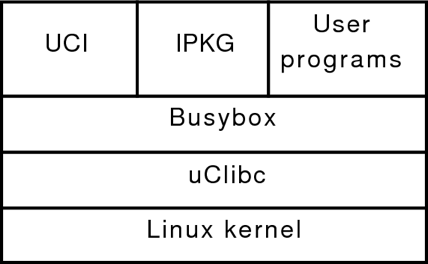
\includegraphics[width=0.4\textwidth]{stack.png}
		\caption{the software stack of OpenWRT}
		\label{OpenWRT:stack}
	\end{figure}
